%--------------------------------------------%
% Template Beamer para Apresentações da UFRN %
% by alcemygvseverino@gmail.com              %
% Baseado em MIT Beamer Template			 %
% versao 1.1								 %
% Atualizado em 14/05/2016					 %
%--------------------------------------------%
\documentclass[handout,t]{beamer}
% Para alterar a linguagem do documento
\usepackage[portuges]{babel}
% Para aceitar caracteres especias deretamente do teclado
\usepackage[utf8]{inputenc}
% Para seguir as normas da ABNT de citacao e referencias
\usepackage[alf]{abntex2cite}
% Para incluir figuras
\usepackage{graphicx}
% Para melhor ajuste da posisao das figuras
\usepackage{float}
% Para ajustar as dimensoes do layout da pagina
\usepackage{geometry}
% Para formatar estrutura e informacoes de formulas matematicas
\usepackage{amsmath}
% Para incluir simbolos especiais em formulas matematicas
\usepackage{amssymb}
% Para incluir links nas referencias
\usepackage{url}
% Para incluir paginas de documentos .pdf externos
\usepackage{pgfpages}
% Para ajustar o estilo dos contadores
\usepackage{enumerate}
% Para modificar a cor do texto
\usepackage{color}
% Para incluir condicoes
\usepackage{ifthen}
% Para colocar legendas em algo que nao e float
\usepackage{capt-of}
% Para definir o tema do slide
\usetheme{Berlin}
% Para difinir cores e background
\usecolortheme{ufrn}
% Para numerar as figuras
\setbeamertemplate{caption}[numbered]
% Para remover o icone padrao antes das referencias
\setbeamertemplate{bibliography item}[text]

% Título
\title[SiameseFWI]{
	SiameseFWI: rede neural siamesa para inversão de forma de onda completa}
% Data
\date{
	Outubro de 2026}
% Autores
\author[Rocha Junior \& Vilar Neto]{
	Ernane Ferreira Rocha Junior \inst{1}\\
	\vspace{0.25cm}
	Pedro Rêgo Vilar Neto \inst{1}}
% Instituto
\institute[PPGEEC/UFRN]{
	\inst{1}%
	Programa de Pós-Graduação em Engenharia Elétrica e de Computação (PPGEEC)\\
	Universidade Federal do Rio Grande do Norte (UFRN)}
% Logo do canto inferior direito
\pgfdeclareimage[height=0.8cm]{logo_ufrn}{figuras/logo_ufrn}
\pgfdeclareimage[height=0.8cm]{logo_lapps}{figuras/logo_lapps}
\pgfdeclareimage[height=0.8cm]{logo_imd}{figuras/logo_imd}
\logo{
	\vspace*{-0.15cm}
	\pgfuseimage{logo_ufrn}
	\pgfuseimage{logo_lapps}
    \pgfuseimage{logo_imd}
	\hspace*{-0.05cm}
    }


\begin{document}
% Sumário
\frame{\titlepage}
\section[]{}
\begin{frame}{Sumário}
	\tableofcontents
\end{frame}

% Introducao
\section{Introdução}

\begin{frame}{O problema: inversão de forma de onda completa}
	\begin{itemize}
		\item \textbf{FWI} (\textit{Full Waveform Inversion}) estima o modelo de velocidade da subsuperfície a partir de dados sísmicos registrados na superfície.
		\item A cada iteração, compara-se o dado simulado com o dado observado e atualiza-se o modelo de velocidade para reduzir essa diferença.
		\item A qualidade da inversão depende fortemente de como essa diferença (função de \textit{misfit}) é medida.
		\item O critério mais comum, a norma $L_2$ ponto a ponto, é sensível a diferenças de fase e leva a mínimos locais (\textit{cycle-skipping}).
	\end{itemize}
\end{frame}

\begin{frame}{Motivação do SiameseFWI}
	\begin{itemize}
		\item Trabalhos anteriores propõem funções de \textit{misfit} alternativas: distância de Wasserstein, correlação cruzada, redes adversárias (FWIGAN), redes pré-treinadas por meta-aprendizagem (ML-misfit).
		\item Essas abordagens ou exigem dados rotulados, ou adicionam custo computacional alto, ou dependem de um treinamento prévio em muitos modelos de velocidade.
		\item \citeonline{saad2024} propõem o \textbf{SiameseFWI}: uma rede neural siamesa, treinada de forma \textit{self-supervised} durante o próprio processo de FWI, com baixo custo computacional adicional.
	\end{itemize}
\end{frame}


% Metodologia
\section{Metodologia}

\begin{frame}{Arquitetura geral do SiameseFWI}
	\begin{columns}[T]
		\column{0.58\textwidth}
		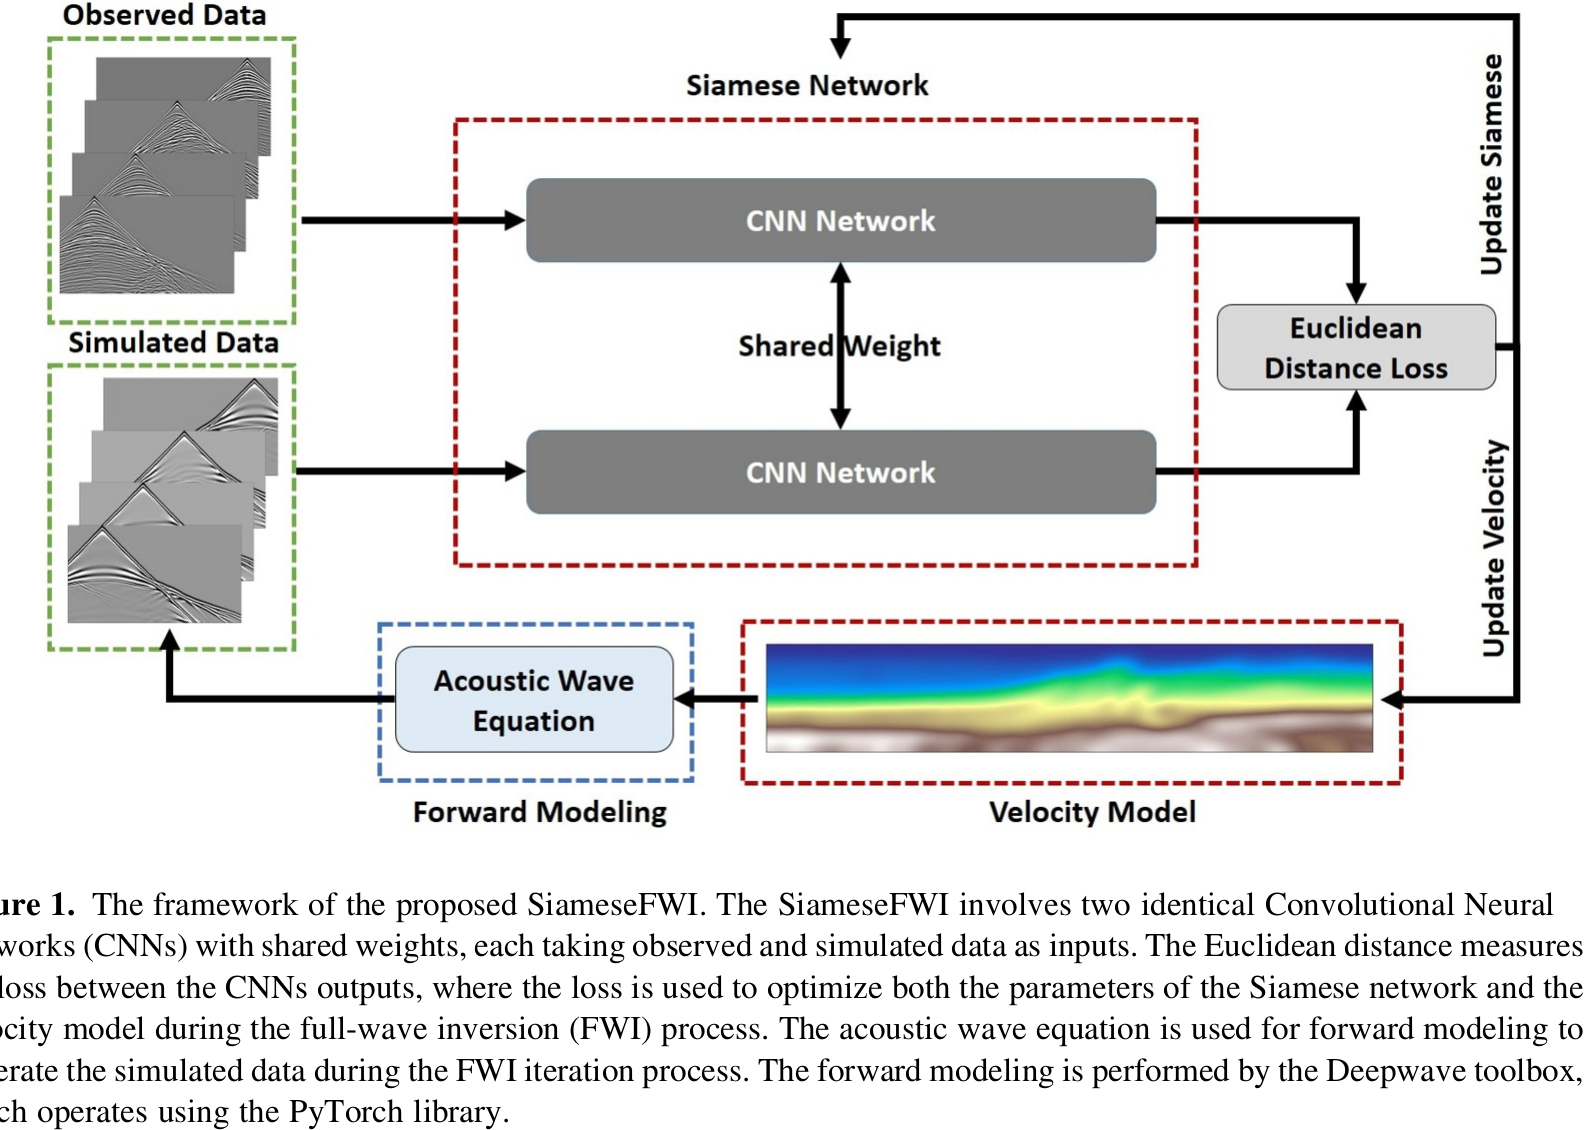
\includegraphics[width=\textwidth]{figuras/paper/fig1_framework}
		\column{0.42\textwidth}
		\begin{itemize}
			\footnotesize
			\setlength{\itemsep}{4pt}
			\item Duas CNNs idênticas, com pesos compartilhados, extraem \textit{features} do dado observado e do dado simulado.
			\item A distância Euclidiana entre as \textit{features} é a perda do SiameseFWI.
			\item Essa perda atualiza, ao mesmo tempo, os pesos da rede siamesa \textbf{e} o modelo de velocidade.
		\end{itemize}
	\end{columns}
\end{frame}

\begin{frame}{Teoria: modelagem direta e função de perda}
	\small
	\setlength{\abovedisplayskip}{4pt}
	\setlength{\belowdisplayskip}{4pt}
	Equação de onda acústica 2D, usada para gerar o dado simulado a cada iteração:
	\begin{equation}
		\nabla^2 p(r,t) = \frac{1}{v^2(r)} \frac{\partial^2 p(r,t)}{\partial t^2} + s(r,t)\,\delta(r - r_s)
	\end{equation}
	Distância Euclidiana entre as \textit{features} extraídas pela rede siamesa, usada como função de perda:
	\begin{equation}
		E = \sqrt{\sum_{i=0}^{n} \big(C(d_{obs}, \phi) - C(d_{sim}, \phi)\big)^2}
	\end{equation}
	\vspace{-0.2cm}
	\begin{itemize}
		\footnotesize
		\item $d_{obs}$ e $d_{sim}$: dado observado e simulado; $C$ e $\phi$: a CNN e seus parâmetros.
		\item Dois otimizadores Adam separados: um para o modelo de velocidade, outro para a rede siamesa.
	\end{itemize}
\end{frame}

\begin{frame}{A rede CNN da arquitetura siamesa}
	\begin{center}
		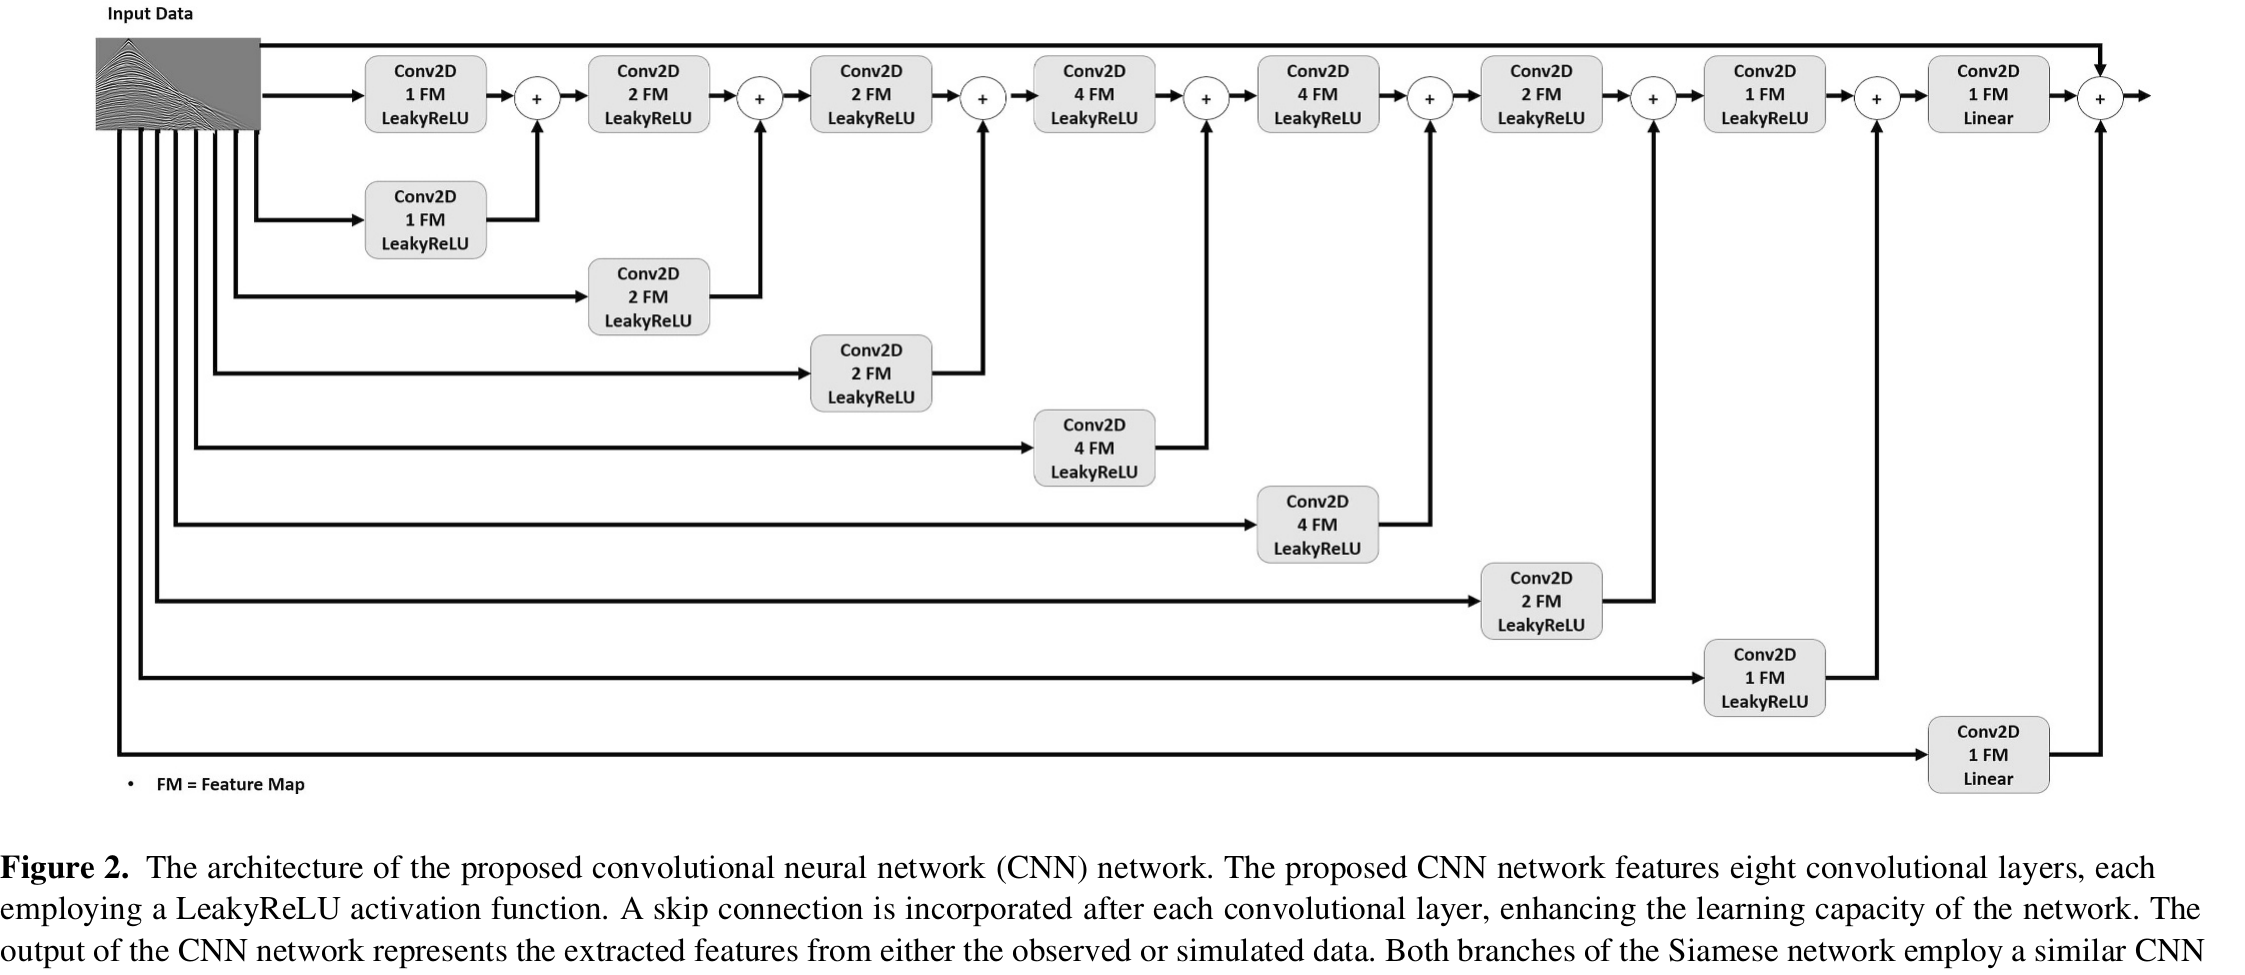
\includegraphics[width=0.95\textwidth]{figuras/paper/fig2_cnn}
	\end{center}
	\begin{itemize}
		\footnotesize
		\item 8 camadas convolucionais 3$\times$3 com LeakyReLU, exceto a última, linear.
		\item 8 conexões residuais (\textit{skip connections}), sem camada de \textit{pooling}: o tamanho espacial da entrada é preservado em toda a rede.
		\item Pesos inicializados aleatoriamente e otimizados ao longo do processo de FWI, sem pré-treinamento.
	\end{itemize}
\end{frame}


% Resultados
\section{Resultados}

\begin{frame}{Modelo sintético Marmousi2}
	\begin{columns}[T]
		\column{0.6\textwidth}
		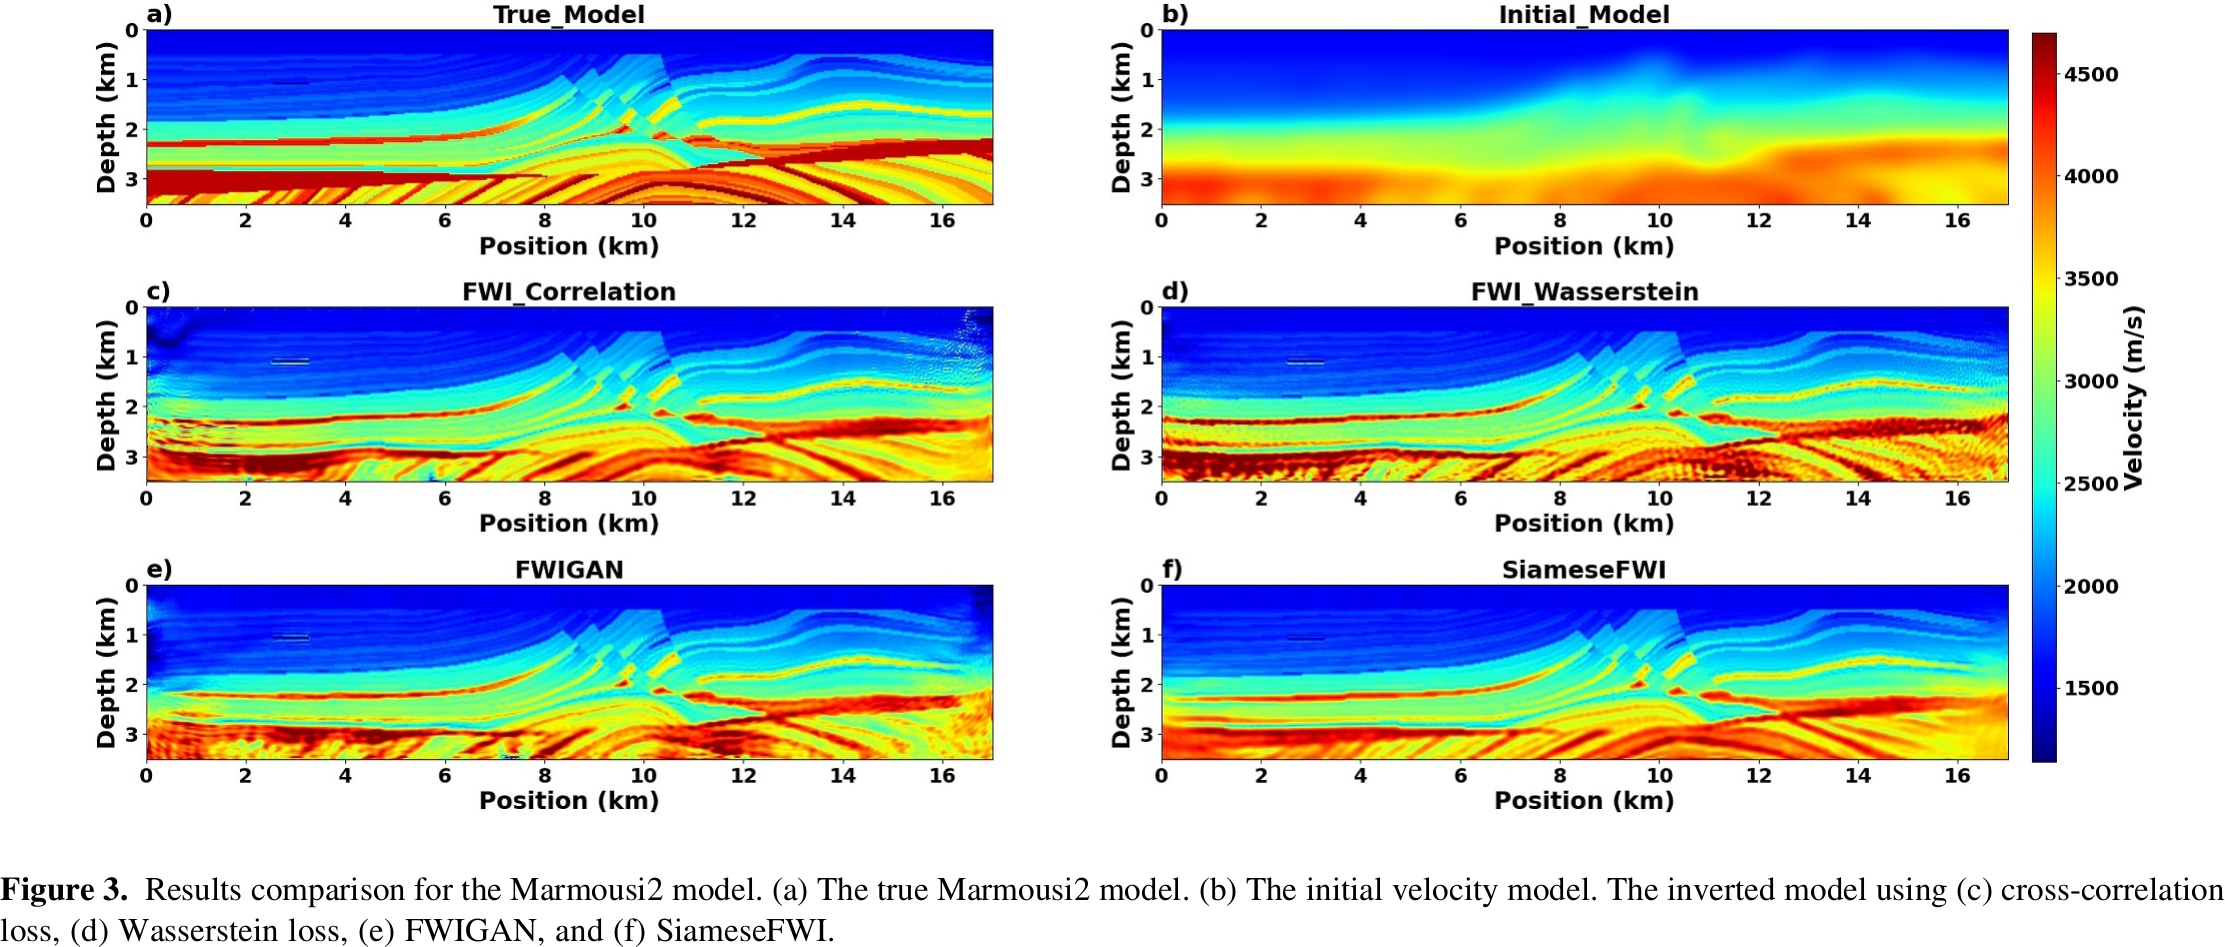
\includegraphics[width=\textwidth]{figuras/paper/fig3_marmousi}
		\column{0.4\textwidth}
		\footnotesize
		\begin{tabular}{lccc}
			\hline
			Método & SNR (dB) & SSIM & RMSE \\
			\hline
			Correlação cruzada & 19,18 & 0,602 & 0,311 \\
			Wasserstein & 19,42 & 0,588 & 0,303 \\
			FWIGAN & 19,06 & 0,583 & 0,316 \\
			\textbf{SiameseFWI} & \textbf{22,57} & \textbf{0,750} & 0,211 \\
			\hline
		\end{tabular}
	\end{columns}
	\vspace{0.2cm}
	\footnotesize SiameseFWI obtém o melhor SNR, SSIM e RMSE entre os quatro métodos, com custo de apenas 10\%--20\% a mais que o FWI convencional.
\end{frame}

\begin{frame}{Modelo sintético Overthrust}
	\begin{columns}[T]
		\column{0.6\textwidth}
		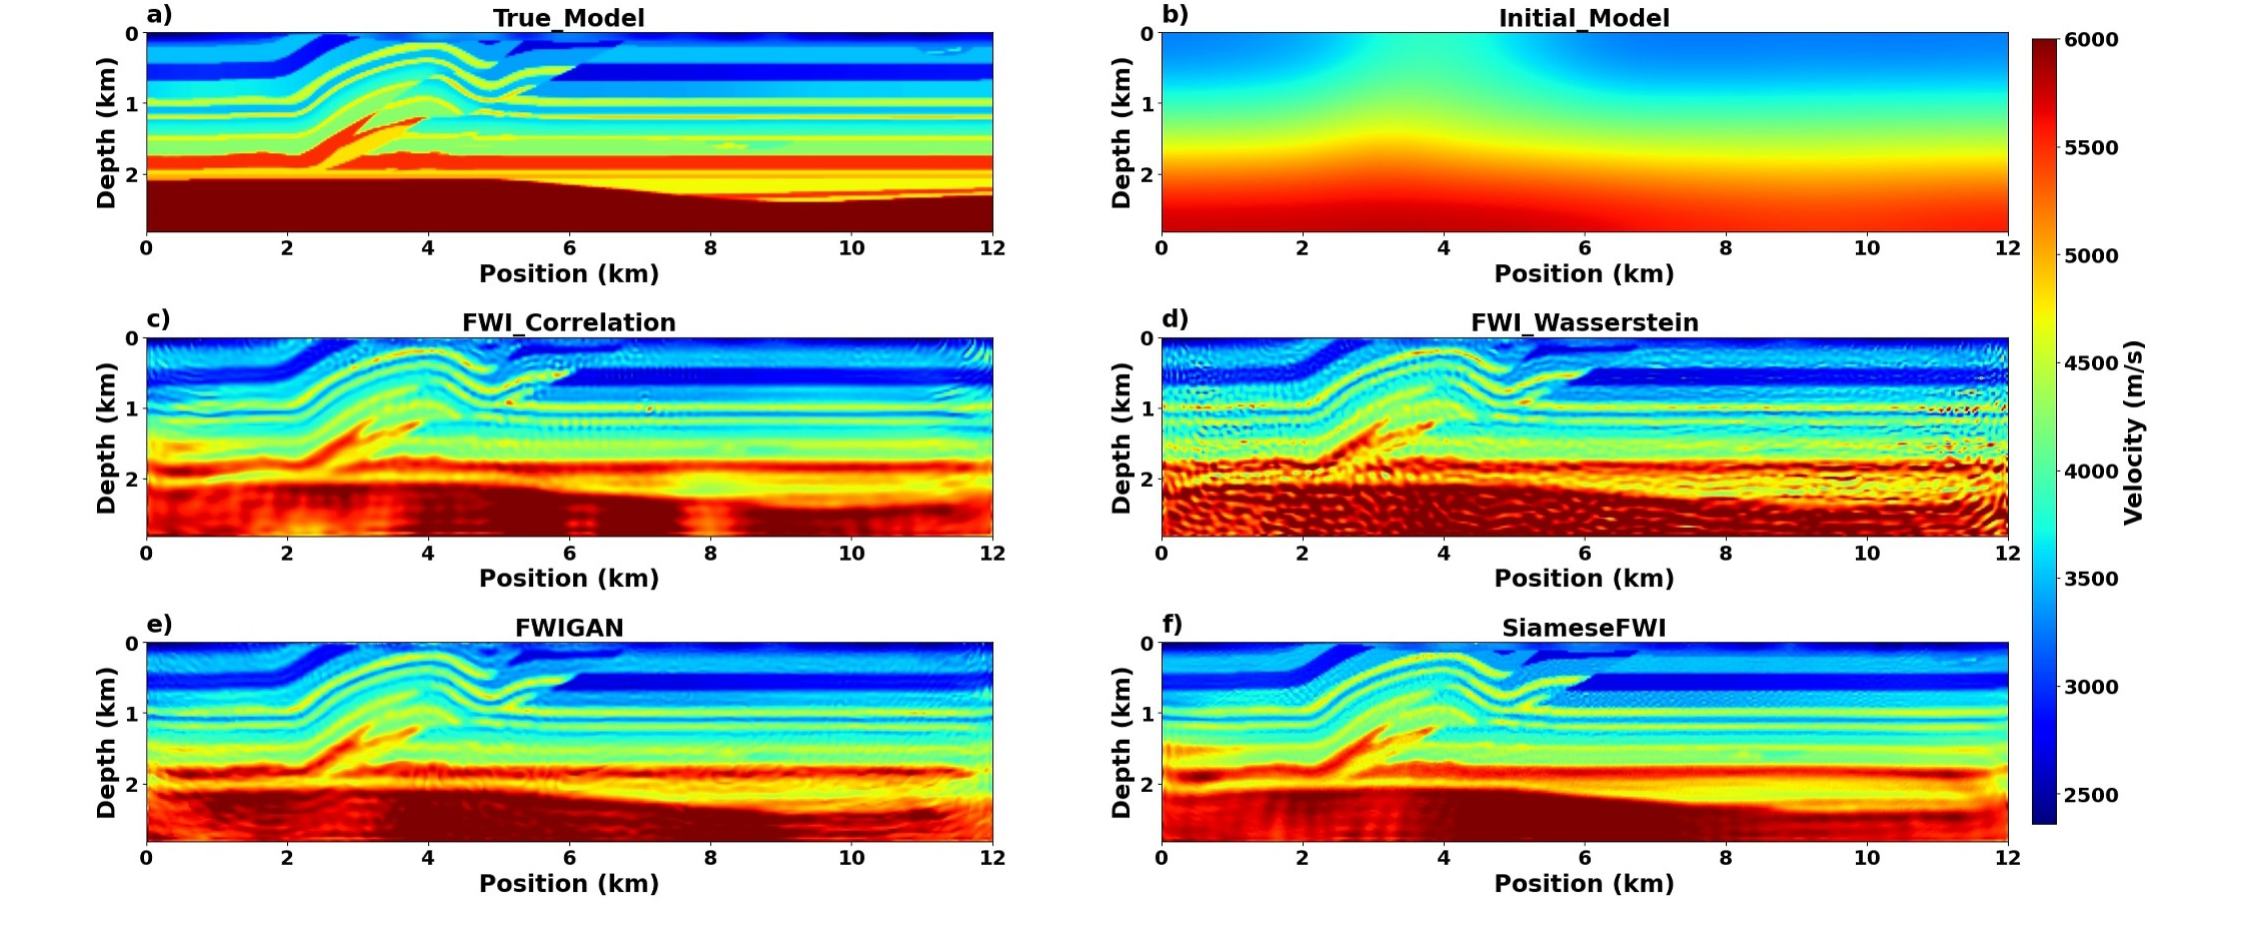
\includegraphics[width=\textwidth]{figuras/paper/fig6_overthrust}
		\column{0.4\textwidth}
		\footnotesize
		\begin{tabular}{lccc}
			\hline
			Método & SNR (dB) & SSIM & RMSE \\
			\hline
			Correlação cruzada & 24,52 & 0,663 & 0,218 \\
			Wasserstein & 23,25 & 0,547 & 0,315 \\
			FWIGAN & 25,95 & 0,663 & 0,228 \\
			\textbf{SiameseFWI} & \textbf{26,98} & \textbf{0,725} & \textbf{0,211} \\
			\hline
		\end{tabular}
	\end{columns}
	\vspace{0.2cm}
	\footnotesize Mesmo padrão do Marmousi2: SiameseFWI à frente em SNR e SSIM, enquanto o FWIGAN (outro método baseado em rede neural) é cerca de 6 vezes mais lento.
\end{frame}

\begin{frame}{Dado de campo (Austrália)}
	\begin{center}
		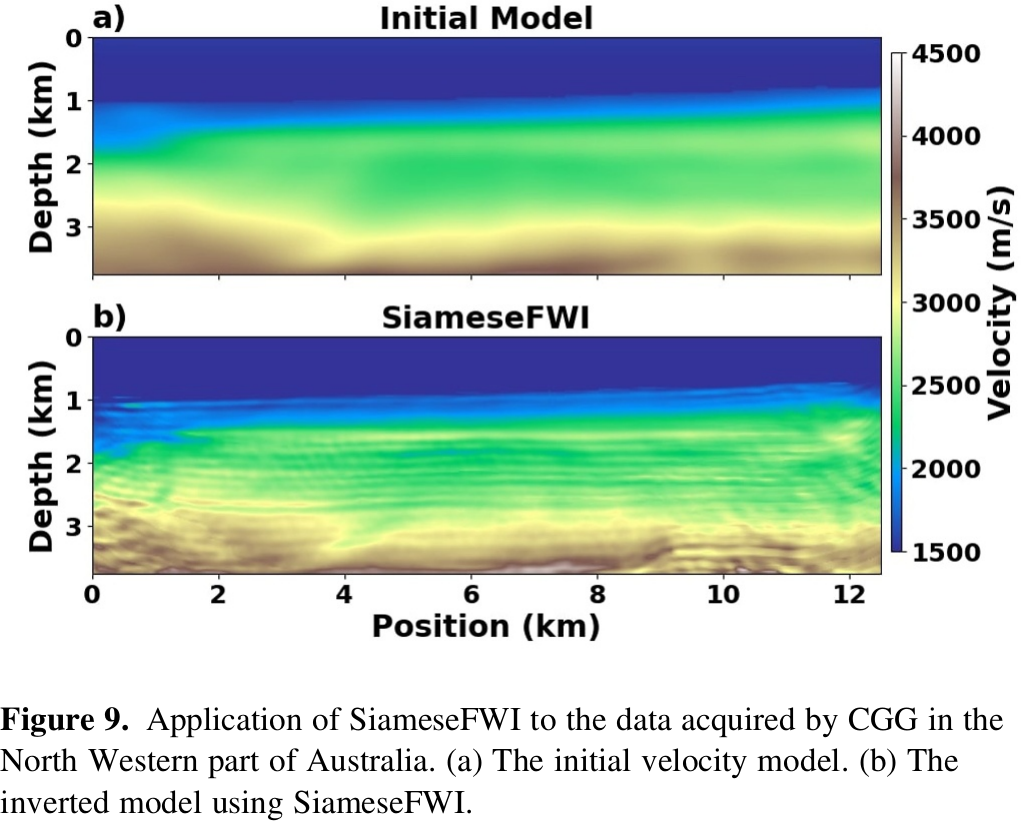
\includegraphics[width=0.34\textwidth]{figuras/paper/fig9_field}
	\end{center}
	\vspace{-0.15cm}
	\begin{itemize}
		\scriptsize
		\setlength{\itemsep}{2pt}
		\item Dado sísmico marinho real, sem modelo de velocidade verdadeiro conhecido.
		\item O modelo invertido pelo SiameseFWI ajusta melhor os dados observados que o modelo inicial, sobretudo nos afastamentos maiores entre fonte e receptor.
		\item Migração reversa no tempo (RTM) com o modelo invertido resolve melhor as interfaces entre 1,5 e 2 km de profundidade.
	\end{itemize}
\end{frame}

\begin{frame}{Robustez do SiameseFWI}
	\begin{itemize}
		\item \textbf{Ruído:} com ruído branco gaussiano aditivo (SNR do dado de $-5$ dB), SiameseFWI mantém SNR de 23,48 dB no modelo invertido, contra 19,18 dB da perda de Wasserstein.
		\item \textbf{Modelo inicial impreciso:} mesmo partindo de um modelo inicial linear (sem nenhuma estrutura real), SiameseFWI converge para um modelo próximo ao verdadeiro.
		\item \textbf{\textit{Wavelet} de fonte desconhecida:} ao estimar a \textit{wavelet} junto com o modelo de velocidade, o método ainda atinge SNR de 24 dB.
	\end{itemize}
\end{frame}


% Conclusao
\section{Conclusão}

\begin{frame}{Limitações e trabalhos futuros}
	\begin{itemize}
		\item Dois otimizadores Adam (rede siamesa e modelo de velocidade) precisam de taxas de aprendizado bem coordenadas entre si.
		\item Sem camada de \textit{pooling}, o tamanho espacial é preservado em toda a rede: em dados de campo de grande dimensão, isso aumenta o custo de memória e processamento.
		\item A rede siamesa aprendida em um conjunto de dados não transfere bem para outro: \textit{transfer learning} direto do Overthrust para o Marmousi2 piora o resultado (SNR cai de 22,57 para 20,27 dB).
	\end{itemize}
\end{frame}

\begin{frame}{Conclusão}
	\begin{itemize}
		\item O SiameseFWI usa uma rede siamesa \textit{self-supervised}, treinada durante o próprio FWI, para comparar dado observado e simulado em um espaço latente.
		\item Supera FWI com perdas convencionais (correlação cruzada, Wasserstein) e o FWIGAN, tanto em modelos sintéticos quanto em dado de campo real.
		\item Alcança esse ganho com apenas 10\%--20\% de custo computacional extra, e se mantém robusto a ruído e a modelo inicial impreciso.
	\end{itemize}
\end{frame}


% Referencias
\section{Referências}
\begin{frame}[allowframebreaks]{Referências}
	\bibliography{bib/bibliografia}
\end{frame}


\end{document}